\chapter{Marco Teórico} \label{chap:marcoteorico}

En el siguiente capitulo se pondrá al alcance del lector las bases teóricas y los conocimientos necesarios para poder entender las diferentes terminologías utilizadas en el trabajo de investigación realizado.

Se tratará de dar un enfoque simplificado de temas como: ¿que es el sensado remoto?, ¿que es el Aprendizaje Automatico?, descripción y desarrollo de Algoritmos de optimización, validación de modelos, Computer Vision.

Para finalizar se expondra la arquitectura, entrenamiento y reconocimiento de objetos a traves de  redes neuronales convolucionales y clasificadores.

\section{Sensado Remoto}\label{sec:sensadoremoto}

En esta sección desarrollaremos el principal enfoque de este trabajo que son las imágenes satelitales; como se forman, rangos de bandas, instrumentos utizados y datos con los cual se trabaja.

\subsection{Teledetección}\label{sub:teledeteccion}

Para comenzar a introducir el concepto de imagen satelital debemos saber como esta formada la misma, es por esto que vamos a desarrollar el concepto de \textit{teledetección}.

La teledeteccion o sensado remoto tambien llamado es el proceso que nos permite obtener una imagen de la superficie terrestre de forma remota, es decir sin estar en contacto con ella. Una imagen satelital es una representación de estos datos reflejados por la superficie terrestre que son captadas por un sensor que se encuentran a bordo de un satélite artificial (ver fig \ref{Fig:teledeteccion}).

En general la teledetección es la medición de energía emanada de la superficie terrestre. Existen diferentes fuentes de energia; si la fuente de energía es el sol entonces lo llamamos \textit{teledetección pasiva}, si la energia medida no es emitida por el Sol, es decir es emitida por un sensor, llamamos \textit{teledetección activa}, como por ejemplo los sensores de radar que funcionan en el rango de microondas.

Los componentes basicos de un sistema de teledetección incluye lo siguiente \citep{chuvieco}:
\begin{itemize}
\item Fuente de energia:

\item Cubierta terrestre:

\item Sistema Sensor:

\item Sistema de Recepción:

\item Interprete

\item Usuario Final
\end{itemize}





La teledeteccion no es mas que la detección de propiedades relevantes del entorno; esta capacidad no es despreciable, nos permite desarrollar aplicaciones practicas con un impacto cada ves mayor \citep{percepcion}. Los datos captados incluyen desde sensores hiperespectrales, multiespectrales, radares, infrarrojos y ópticos.

\begin{center} \begin{minipage}{0.8\linewidth}  \vspace{5pt} {\small
Either to supplement the capability of sensors or to effectively utilize the enormous amount of sensor data, many advances in statistical pattern recognition can be very useful in machine recognition of the data. The potentials and opportunities of using statistical pattern recognition in remote sensing are indeed unlimited.}
\begin{flushright} (\citeauthor{Ledda})
\end{flushright}
\end{minipage}
\end{center}

\begin{figure}[H] \centering
  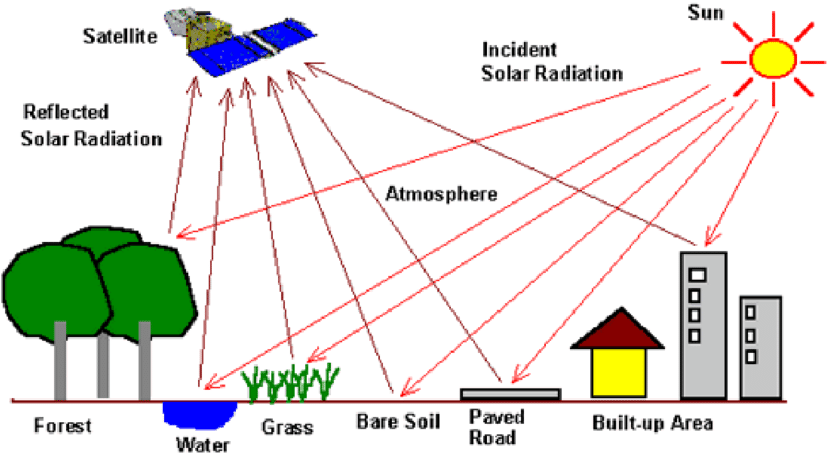
\includegraphics[height=8cm,keepaspectratio=true,clip=true]{imagenes/MarcoTeorico/teledeteccion.png}
  \caption{Sensado Remoto. Navarrete, Edison, Laubacher, Gerard}\label{Fig:teledeteccion}
\end{figure}

Esta disciplina es una las áreas de mayor interés y crecimiento de los últimos años dentro de la informática en el procesamiento de imágenes. La clasificación de imágenes es una de las mayores tareas a la hora de realizar el procesamiento de  las imágenes satelitales y es donde vamos a poner nuestro mayor esfuerzo.










